\documentclass[8pt,a4paper,ngerman]{scrartcl}
\usepackage[utf8]{inputenc}
\usepackage{hyperref}
\usepackage{geometry}
\usepackage{graphicx}
\geometry{a4paper, top=15mm,left=30mm,right=30mm,bottom=25mm,headsep=10mm,footskip=12mm}

\begin{document}
\begin{center}
    \LARGE{\textbf{Exposé zur Bachelorabeit}}
\end{center}
\begin{center}
    \large{Christopher Pahl}
\end{center}
\begin{center}
    \small{\today}
\end{center}

\section{Motivation}
    Heutzutage gibt es viele Plattformen die dabei helfen wollen neue Musik zu
    entdecken. Eine dieser Plattformen ist beispielsweise
    \url{https://www.last.fm}. Nutzer bekommen dabei
    basierend auf ihrem Hörverhalten Vorschläge was sie als nächstes anhören
    könnten - leider ist die Software in ihrem Kern keine \emph{FOSS} und zudem
    abhängig von den zentralen Servern des Betreibers. Daher wäre ein freies,
    clientseitiges System wünschenswert.
    \\
    \\
    Die Zielgruppe wären hierbei Entwickler von Musicplayern oder vergleichbarer
    Software. Auch ein \emph{Standalone-Tool} wäre denkbar welches von normalen Usern
    genutzt werden kann.

\section{Themenstellung}
    Erstellen einer Softwarebibliothek zur automatisierten Empfehlung von Musik
    basierend auf der Musik-Sammlung eines Nutzers und dessen Hör-Gewohnheiten.
    \\
    \\
    Im Speziellen soll das System dabei die Musik-Datenbank des Nutzers importieren
    und dessen Hör-Gewohnheiten beobachten können. Daraus sollen dann
    Empfehlungen (\textit{N} ähnliche Songs zu Stück \textit{X}) und Dynamische Playlisten 
    (Playlist die zu den zuletzt Gehörtem passt) abgeleitet werden können.
    \\
    \\
    Beteiligte Disziplinen der Informatik:

    \begin{itemize}
        \item Graphentheorie (Aufbau/Wartung der internen Graphenstruktur)
        \item Datamining-Algorithmen (Ähnlichkeitsmaß, Machinenlernende Systeme)
        \item Maschinelles Lernen (Prüfen ob Empfehlungen angenommen wurden)
        \item Audioanalyse (Moodbar (siehe Literatur [\ref{label_moodbar})])
    \end{itemize}

    \subsection{Namensgebung:}

        Die Library soll \emph{libmunin} heißen, wie Odin's Rabe \emph{Munin}:

        \begin{quote}
            \textit{Munin gehört zum altnordischen Verb muna (denken an, sich erinnern), 
            der Name Munin bedeutet folglich ,,die Erinnerung''.}
        \end{quote}

        Siehe auch: \url{http://de.wikipedia.org/wiki/Hugin_und_Munin}

\section{Geplantes Vorgehen}
    Es soll eine Prototyp für unixoide Betriebssysteme in \emph{Python}
    implementiert werden. Wenn noch
    ausreichend Zeit bleibt (leider eher unwahrscheinlich) soll dieser Prototyp in eine
    \emph{C-Bibliothek} umgesetzt werden. Zuerst soll die Grundfunktionalität der
    Bibliothek stehen, danach können dann \emph{spezielle Provider}, welche
    beispielsweise eine \emph{Moodbar-Anaylse} oder \emph{Liedtexte vergleichen}, implementiert
    werden. Wenn die Library rechtzeitig in einem annehmbaren Zustand sein, so soll
    die Library in einem \emph{MPD-Client zum Einsatz} kommen. 
    \\
    \\
    Später soll dann die \emph{Theorie} mit Zuhilfenahme von \emph{Visualisierungen} detailliert in 
    der Bachelor-Arbeit beschrieben werden und, nach Möglichkeit, wird das System an 
    \emph{echten Menschen} und verschiedenen Musik-Sammlungen getestet um zu
    sehen ob es auch praxistauglich ist.

\section{Aufteilung/Zeitplanung}
    Relative Zeitabschätzung in (Klammern):

    \paragraph{Projektarbeit:}
        \begin{enumerate} 
            \item Implementierung von \emph{libmunin}. (ca. 55\%)
            \item {[}\emph{Optional}{]} Beispielanwendung in einem MPD-Client (voraussichtlich
                ,,\emph{Moosecat}''). (ca. 15\%)
        \end{enumerate}

    \paragraph{Bachelorarbeit:}
        \begin{enumerate} 
            \item Beschreibung der Theorie/Algorithmik mit Visualisierungen.  (ca. 25\%)
            \item {[}\emph{Optional}{]} Test mit echten Nutzern und verschiedenen
                Musik-Sammlungen. (ca. 5\%)
        \end{enumerate}

\section{Literatur}
    \begin{enumerate}
        \item \textit{Moodbar} (\url{http://cratoo.de/amarok/ismir-crc.pdf}) \label{label_moodbar}
        \item \textit{A Mood Based Music Classification and Exploration System} (\url{http://www.google.de})
        \item \textit{Automatic Playlist Generation via Music Mood Analysis} (\url{http://www.google.de})
        \item \textit{Polysound} (\url{http://grupoweb.upf.edu/~luca.chiarandini/personal/v0/index.html#projectsPolysound})
    \end{enumerate}
\newpage
\begin{figure}[p]
    \vspace*{+1.0cm}
    \hspace*{-3.0cm}
    \rotatebox{270}{\makebox[\linewidth]{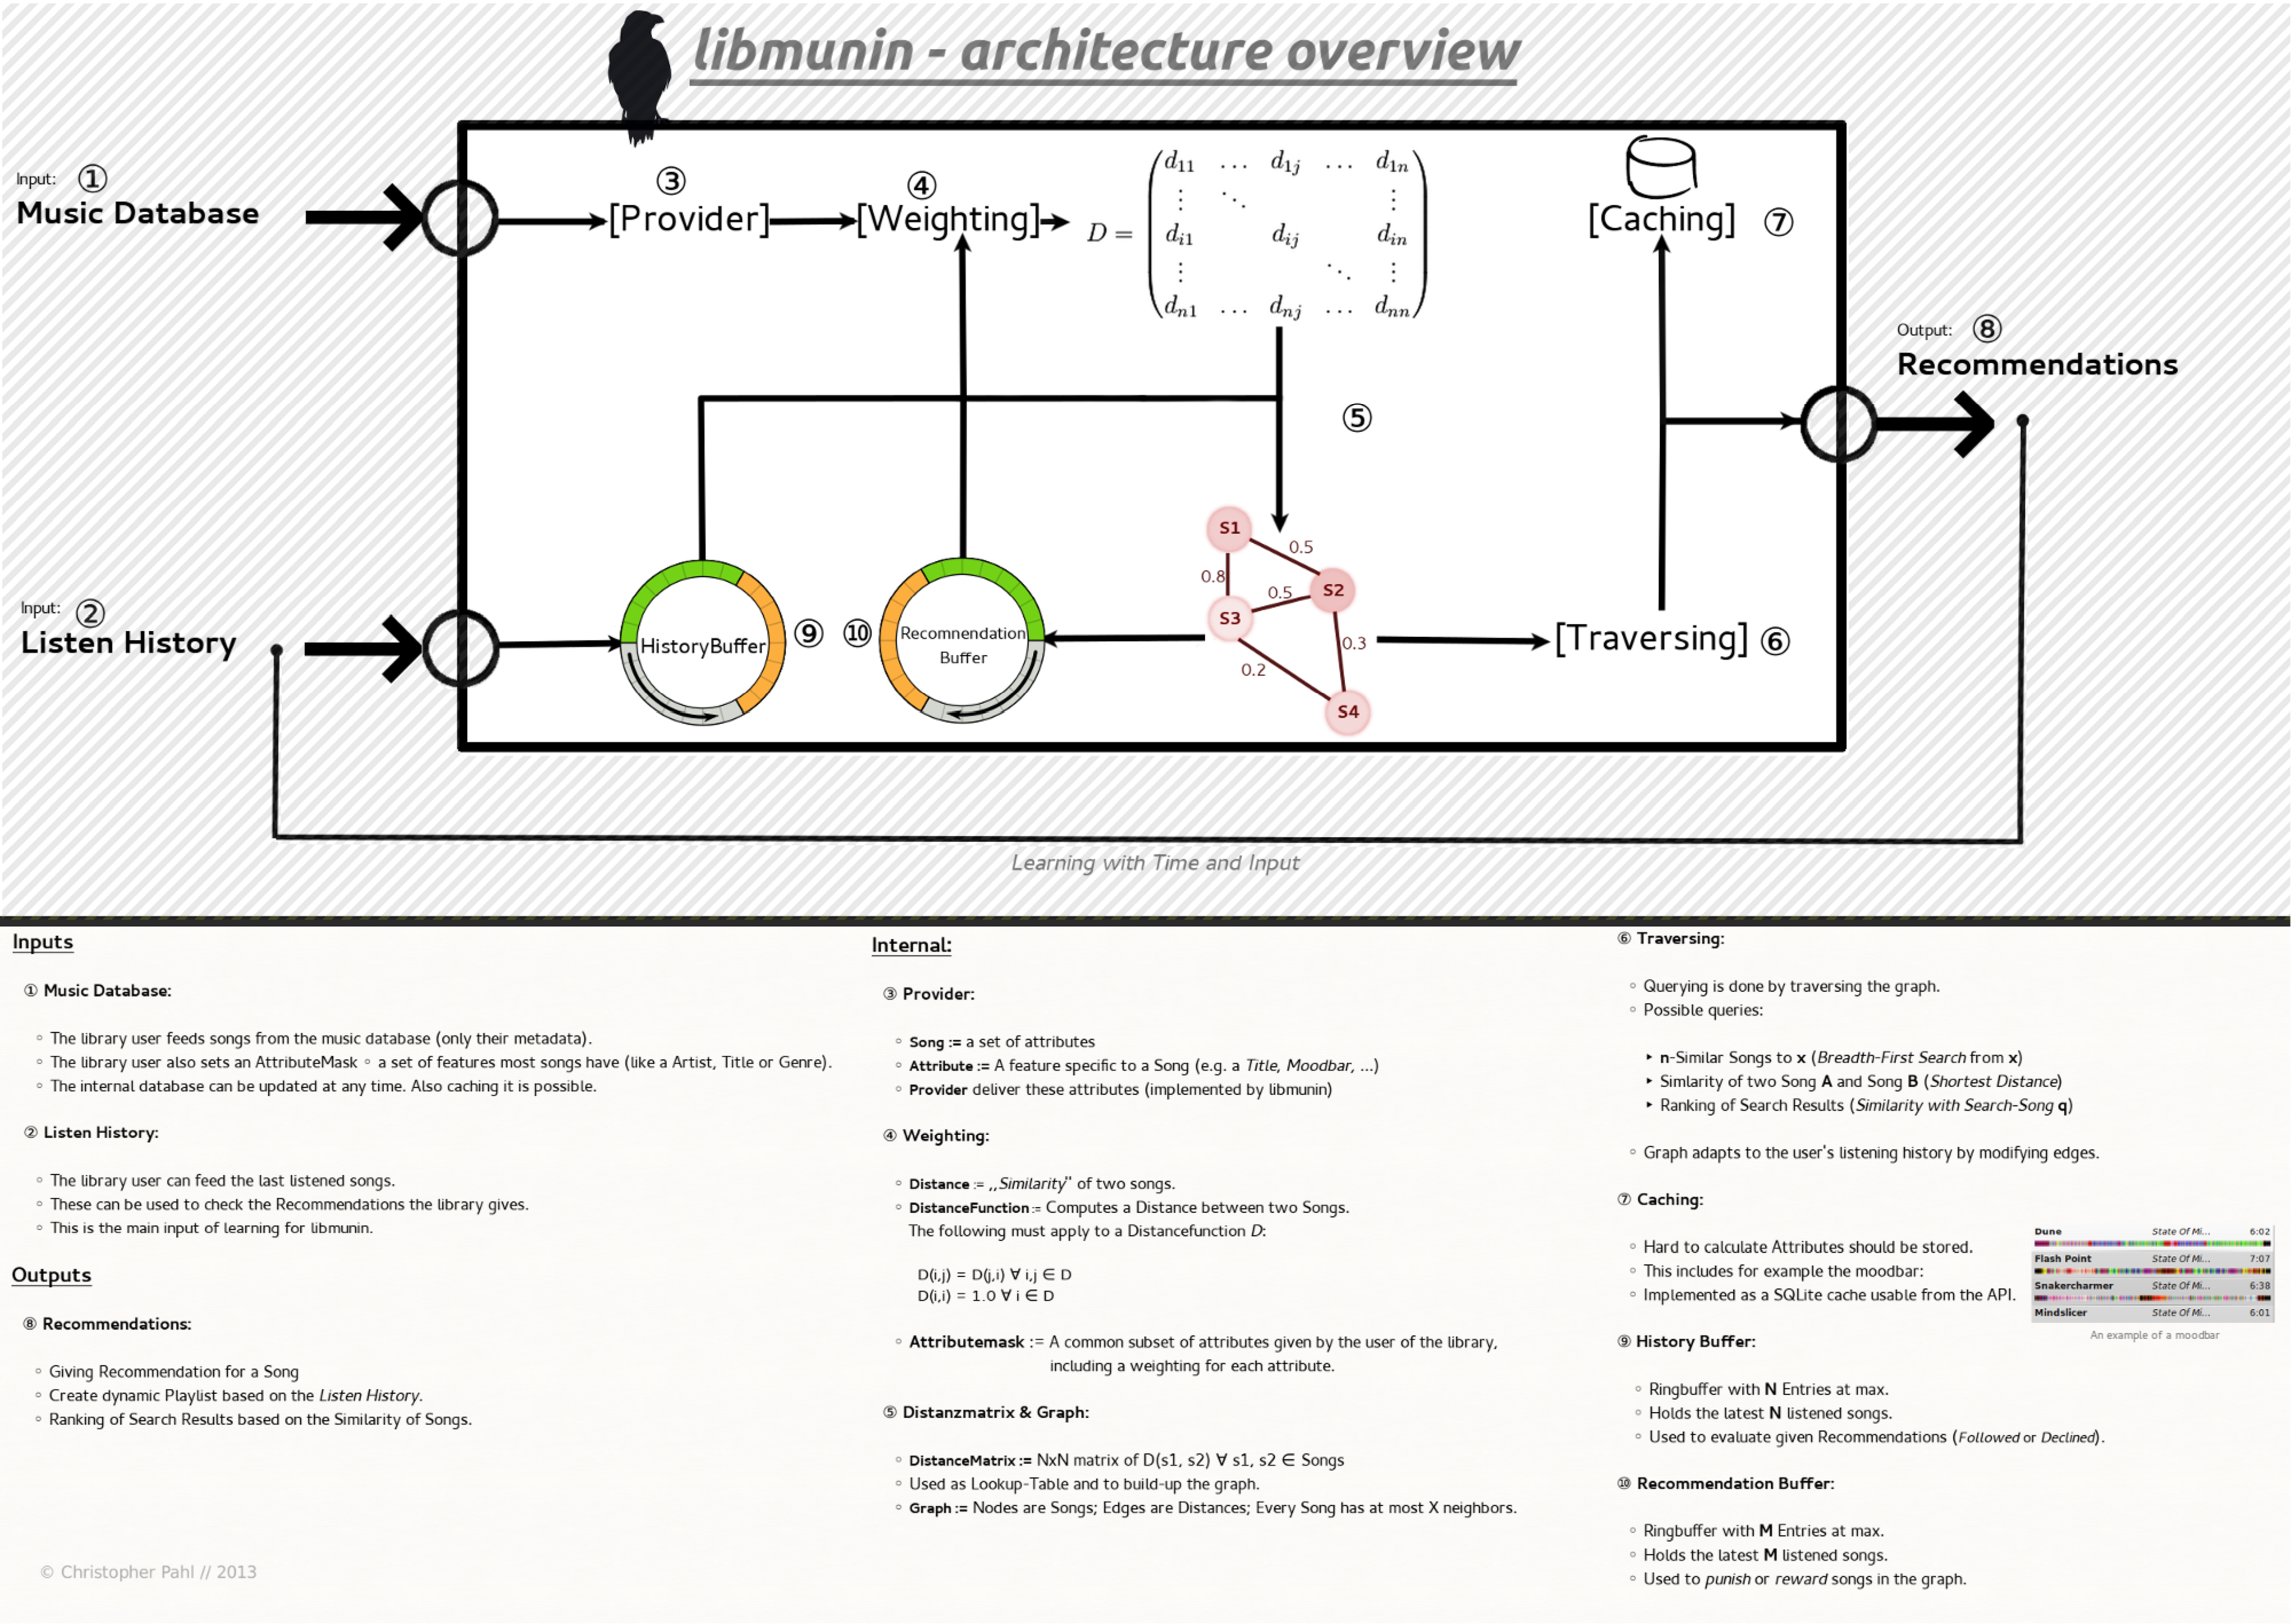
\includegraphics[width=1.97\linewidth]{arch.pdf}}}
\end{figure}

\end{document}
